\section{Herbie: Improving Floating Point Accuracy}
\label{sec:herbie}

Herbie automatically improves accuracy
  for floating-point expressions,
  using random sampling to measure error,
  a set of rewrite rules for generating program variants,
  and algorithms that prune and combine program variants
  to achieve minimal error.
Herbie received PLDI 2015's Distinguished Paper award~\cite{herbie}
  and has been continuously developed since then,
  sporting hundreds of Github stars, hundreds of downloads,
  and thousands of users on its online version.
Herbie uses \egraphs for algebraic simplification of mathematical expressions,
  which is especially important for avoiding floating-point errors
  introduced by cancellation, function inverses, and redundant computation.

Until our case study,
  Herbie used a custom \egraph implementation
  written in Racket (Herbie's implementation language)
  that closely followed traditional \egraph implementations.
With timeouts disabled,
  \egraph-based simplification consumed
  the vast majority of Herbie's run time.
As a fix, Herbie sharply limits the simplification process,
  placing a size limit on the \egraph itself and a time limit on the whole
  procedure.
When the timeout is exceeded, simplification fails altogether.
Furthermore, the Herbie authors knew of several features
  that they believed would improve Herbie's output
  but could not be implemented because
  they required more calls to simplification
  and would thus introduce unacceptable slowdowns.
Taken together, slow simplification reduced Herbie's performance, completeness,
  and efficacy.

We implemented a \egg simplification backend for Herbie.
The \egg backend is over $3000\times$ faster than Herbie's initial simplifier and
  is now used by default as of Herbie 1.4.
Herbie has also backported some of \egg's features like batch simplification and
  rebuilding to its \egraph implementation
  (which is still usable, just not the default),
  demonstrating the portability of \egg's conceptual improvements.
% This has led to over a $200\times$ speedup over its initial design,
%   demonstrating that \egg's

\subsection{Implementation}

Herbie is implemented in Racket while \egg is in Rust;
  the \egg simplification backend is thus implemented as a Rust library that
  provides a C-level API for Herbie to access via foreign-function interface (FFI).
The Rust library defines the Herbie expression grammar
  (with named constants, numeric constants, variables, and operations)
  as well as the \eclass analysis necessary to do constant folding.
The library is implemented in under 500 lines of Rust.

Herbie's set of rewrite rules is not fixed;
  users can select which rewrites to use using command-line flags.
Herbie serializes the rewrites to strings,
  and the \egg backend parses and instantiates them on the Rust side.

Herbie separates exact and inexact program constants:
  exact operations on exact constants
  (such as the addition of two rational numbers)
  are evaluated and added to the \egraph,
  while operations on inexact constants or that yield inexact outputs
  are not.
We thus split numeric constants in the Rust-side grammar
  between exact rational numbers and inexact constants,
  which are described by an opaque identifier,
  and transformed Racket-side expressions into this form
  before serializing them and passing them to the Rust driver.
To evaluate operations on exact constants,
  we used the constant folding \eclass analysis
  to track the ``exact value'' of each \eclass.%
\footnote{Herbie's rewrite rules guarantee that different exact values
  can never become equal; the semilattice \textsf{join} checks this invariant on the Rust side.}
Every time an operation \enode is added to the \egg \egraph,
  we check whether all arguments to that operation have exact value (using the analysis data),
  and if so do rational number arithmetic to evaluate it.
The \eclass analysis is cleaner than the corresponding code in Herbie's implementation,
  which is a built-in pass over the entire \egraph.

\subsection{Results}

\begin{figure}
  \centering
  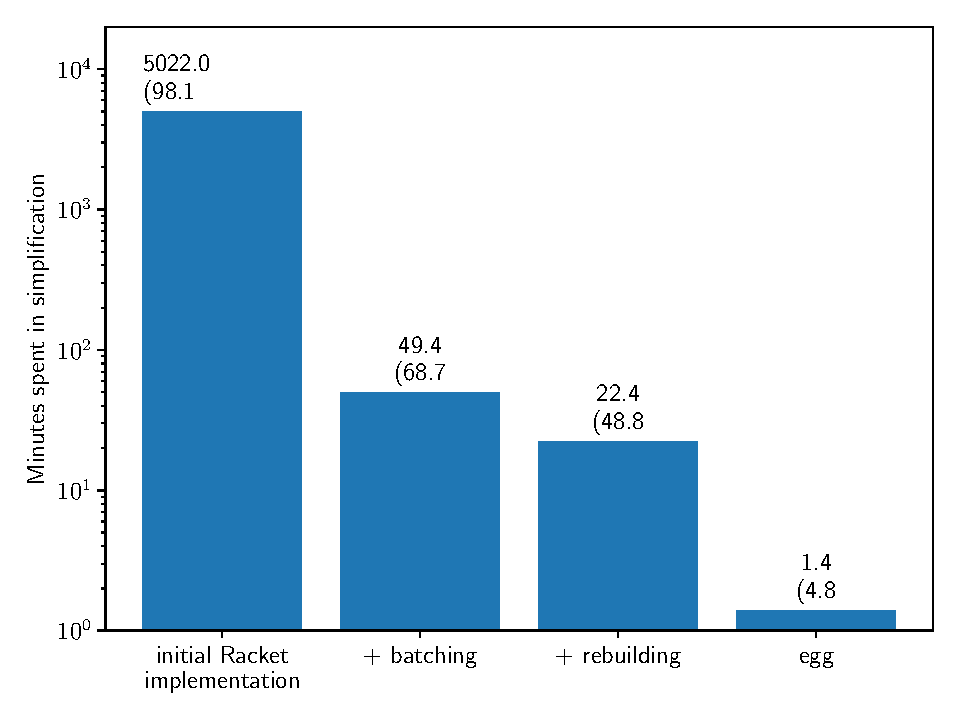
\includegraphics[height=8cm]{herbie}
  \caption{
    Herbie sped up its expression simplification phase
      by adopting \egg-inspired features like
      batched simplification and rebuilding
      into its Racket-based \egraph implementation.
    Herbie also supports using \egg itself for additional speedup.
    Note that the y-axis is log-scale.
  }
  \label{fig:herbie-results}
\end{figure}

Our \egg simplification backend
  is a drop-in replacement to the existing Herbie simplifier,
  making it easy to compare speed and results.
We compare using
  Herbie's standard test suite of roughly 500 benchmarks,
  with timeouts disabled.
\autoref{fig:herbie-results} shows the results.
The \egg simplification backend is over
  $3000\times$ faster than Herbie's initial simplifier.
This speedup eliminated Herbie's largest bottleneck:
  the initial implementation dominated Herbie's total run time at $98.1\%$,
  backporting \egg improvements into Herbie cuts
  that to about half the total run time,
  and \egg simplification takes under $5\%$ of the total run time.
Practically, the run time of Herbie's initial implementation was smaller, since
  timeouts cause tests failures when simplification takes too long.
Therefore, the speedup also improved Herbie's completeness,
  as simplification now never times out.

Since incorporating \egg into Herbie, the Herbie developers have backported some
  of \egg's key performance improvements into the Racket \egraph implementation.
First, batch simplification gives a large speedup because Herbie simplifies many
  similar expressions.
When done simultaneously in one equality saturation, the \egraph's structural
  sharing can massively deduplicate work.
Second, deferring rebuilding (as discussed in \autoref{sec:rebuilding}) gives a
  further $2.2\times$ speedup.
As demonstrated in \autoref{fig:eval-iter}, rebuilding offers an asymptotic
  speedup, so Herbie's improved implementation (and the \egg backend as well)
  will scale better as the search size grows.

%%% Local Variables:
%%% TeX-master: "../thesis"
%%% End: